\begin{figure}[t]
\centering
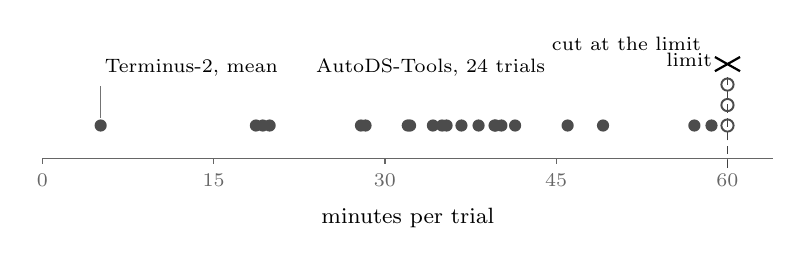
\begin{tikzpicture}[x=0.145cm,y=1cm]
\draw[black!60] (0,0) -- (64,0);
\draw[black!60] (0,0) -- (0,-0.07) node[below,font=\scriptsize,black!60]{0};
\draw[black!60] (15,0) -- (15,-0.07) node[below,font=\scriptsize,black!60]{15};
\draw[black!60] (30,0) -- (30,-0.07) node[below,font=\scriptsize,black!60]{30};
\draw[black!60] (45,0) -- (45,-0.07) node[below,font=\scriptsize,black!60]{45};
\draw[black!60] (60,0) -- (60,-0.07) node[below,font=\scriptsize,black!60]{60};
\node[font=\footnotesize,anchor=north] at (32,-0.5){minutes per trial};
\draw[densely dashed,black!75] (60.0,-0.12) -- (60.0,1.05);
\node[font=\scriptsize,anchor=south east] at (60.0 - 0.5,1.05){limit};
\fill[black!70] (18.7,0.42) circle (2.2pt);
\fill[black!70] (19.3,0.42) circle (2.2pt);
\fill[black!70] (19.9,0.42) circle (2.2pt);
\fill[black!70] (27.9,0.42) circle (2.2pt);
\fill[black!70] (28.3,0.42) circle (2.2pt);
\fill[black!70] (32.0,0.42) circle (2.2pt);
\fill[black!70] (32.2,0.42) circle (2.2pt);
\fill[black!70] (34.2,0.42) circle (2.2pt);
\fill[black!70] (35.0,0.42) circle (2.2pt);
\fill[black!70] (35.4,0.42) circle (2.2pt);
\fill[black!70] (36.7,0.42) circle (2.2pt);
\fill[black!70] (38.2,0.42) circle (2.2pt);
\fill[black!70] (39.6,0.42) circle (2.2pt);
\fill[black!70] (39.7,0.42) circle (2.2pt);
\fill[black!70] (40.2,0.42) circle (2.2pt);
\fill[black!70] (41.4,0.42) circle (2.2pt);
\fill[black!70] (46.0,0.42) circle (2.2pt);
\fill[black!70] (49.1,0.42) circle (2.2pt);
\fill[black!70] (57.1,0.42) circle (2.2pt);
\fill[black!70] (58.6,0.42) circle (2.2pt);
\draw[black!70,line width=0.7pt] (60.0,0.42) circle (2.2pt);
\draw[black!70,line width=0.7pt] (60.0,0.6799999999999999) circle (2.2pt);
\draw[black!70,line width=0.7pt] (60.0,0.94) circle (2.2pt);
\draw[black,line width=0.8pt] (60.0-1.1,1.2-0.09+0.0) -- (60.0+1.1,1.2+0.09+0.0) (60.0-1.1,1.2+0.09+0.0) -- (60.0+1.1,1.2-0.09+0.0);
\node[font=\scriptsize,anchor=east,xshift=-6pt] at (60.0,1.46) {cut at the limit};
\fill[black!70] (5.1,0.42) circle (2.2pt);
\draw[black!55] (5.1,0.52) -- (5.1,0.92);
\node[font=\scriptsize,anchor=south west,xshift=-2pt] at (5.1,0.92){Terminus-2, mean};
\node[font=\scriptsize,anchor=south] at (34,0.92) {AutoDS-Tools, 24 trials};
\end{tikzpicture}
\caption{Agent wall-clock per trial on TabReD. Each filled dot is an AutoDS-Tools trial that finished on its own. Four did not: they were cut at the task's own limit, and the distinction that matters is what was on disk at that moment. Three (open circles) had already written a submission and are scored like any other trial; one (cross) had not, and is the only trial we lose. The open harness averages five minutes on the same tasks under the same limit.}
\label{fig:walltime}
\end{figure}
